\section{Artificial Intelligence}
Als \ac{AI} oder im deutschen auch \emph{artifizielle Intelligenz} oder \emph{k�nstliche Intelligenz}, bezeichnet, in der Informatik, ein System welches eine Automatisierte Intelligenz besitzt. Eine eindeutige Definition f�r \ac{AI} gibt es nicht, da es schon in der Psychologie an einer genauen Definition mangelt. \cite{WikiKI}

In der heutigen Zeit werden Systeme und Algorithmen die auf neuronalen Netzen basieren als ann�hernd intelligent bezeichnet. Ein Beispiel hierf�r ist "`Google Translate"' welches zwischen verschiedenen Sprachen mittels neuronalen Netz �bersetzt. \cite{TranslateKI}

Es gibt aber auch intelligente Systeme wie "`IBM Watson"', welche nicht auf neuronalen Netzen basieren und ann�hernd intelligent wirken. Diese Intelligenz ist das Resultat einer sehr gro�en Wissensbasis und verschiedenen kombinatorischen Algorithmen. Um zu zeigen wie Leistungsf�hig Watson ist, trat er 2011 in der Quizshow "`Jeopardy"' an und gewann gegen die weltbesten Spieler. \cite{IBMWatson}

Im allgemeinen Sprachgebrauch werden als \ac{AI} heute �blichen Sprachassistenten wie Siri, Alexa, Cortana oder Google Assistent bezeichnet. Das im Verlauf der Arbeit zu entwickelnde \ac{NUI} soll auf einen dieser Assistenten aufbauen.

Die Entwicklung einer eigenen Spracherkennung ist im Rahmen dieser Arbeit nicht m�glich, da dies sehr viel Zeit und Arbeit in Anspruch nimmt. Selbst Firmen wie Google oder Amazon ben�tigten mehrere Jahre um ihre Assistent auf das aktuelle Leistungsniveau zu heben.

Es soll nun untersucht werden, in wie weit die heute g�ngigen Assistenten genutzt werden k�nnen, um eine Sprachsteuerung f�r ein \ac{NUI} (siehe Kapitel ?????) umzusetzen.

Hierbei muss der Assistent folgende Kriterien erf�llen:
\begin{itemize}
 \item Lauff�gig auf der Microsoft HoloLens
 \item Offene Programmierschnittstelle (\ac{SDK})
 \item M�glichkeit eigener Sprachkomandos
\end{itemize}

\subsection{Funktionsweise der Sprachassistenten}
Auch wenn die genauen Implementierungen der Sprachassistenten verschiedenen ist, so haben sie alle eins gemenisam und zwar ist dies der Weg der Sprachverarbeitung.

Die Funktionsweise von Siri udn Co. ist recht einfach gehalten. Der Nutzer l�st mit einem Stichwort "`Hey, Siri..."', "`Ok, Google..."' und so weiter die Benutzung aus. Der darauf folgende Sprachbefehl wird aufgezeichnet und komprimiert an einen Server weitergeleitet, welcher den gesprochenen Text auswertet und in schriftliche Befehle umwandelt. Diese Befehle werden dann umgehend zur�ck an das Endger�t des Nutzers Versand, welches nun auf die Befehle reagieren kann.

\begin{figure}[!ht]
\centering
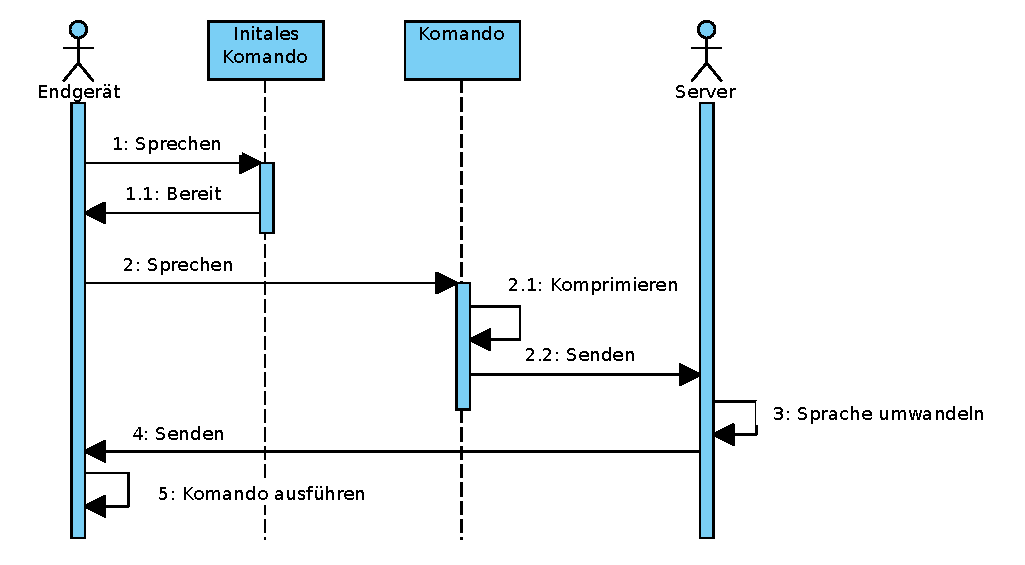
\includegraphics[width=14cm]{Bilder/Assistenten.eps}
\caption{Schematische Darstellung der Kommunikation von Sprachassistenten}
\label{assistent_img}
\centering
\end{figure}

Hierbei ist zu beachten, dass jegliche Kommunikation zwischen Endger�t und Server bei allen Assistenten �ber HTTPS gesichert ist.

Innerhalb der Server, welche die Sprache zu Text wandeln, kommen fast immer neuronale Netze zum einsatz, da nur sie in der Lage sind schnell und eindeutig die Spachbefehle zu wandeln.
Durch die geh�ufte Verwendung mit immer neuen Stimmen und Befehlen lernen die Systeme immer mehr hinzu und k�nnen so die Anfragen immer schneller und besser umwandeln. Dies hat zur Folge, das ein System besser wird, je h�ufiger es genutzt wird.

In den nun folgenden Abschnitten werden die genannten Assistenten auf ihre M�glichkeiten untersucht.

\subsection{Siri}
Der wohl �lteste und bekannteste Sprachassistent ist "`Siri"'. Siri ist eine Software zur Spracherkennung und wurde von Apple im Jahre 2010 zusammen mit der Firma Siri Inc. von Apple aufgekauft. Schon ein Jahr sp�ter wurde der Assistent im Zuge der Ver�ffentlichung des iPhone 4s vorgestellt und ver�ffentlicht.

Siri ist eine propriet�re Software und nur iOS, machOS, watchOS und tvOS einsetzbar, weshalb eine Verwendung auf der HoloLens nicht m�glich ist. Zwar verf�gt Siri �ber ein offenes \ac{SDK}, dieses ist jedoch nur f�r Apple eigene Betriebssysteme ausgelegt.


\subsection{Alexa}
\subsection{Cortana}
\subsection{Google Assistent}

\subsection{Auswertung der M�glichkeiten}
